\chapter{智能，生于数学 \texorpdfstring{\\}{ }简明数学史}

%{\newenvironment{examplebox}
%{\par\vspace{0.5em}\noindent\hrulefill\par\noindent{示例盒子：三跳链}\par\small}
%{\par\noindent\hrulefill\vspace{0.5em}\normalsize\par}
%}

\begin{introduction}
\item 萌芽：从结绳计数到位值制（建立“可表示与可计算”的底座）
\item 初等：几何、公理化与证明（从计算转向论证）
\item 近代：变量、函数、微积分与解析几何（刻画变化与空间）
\item 现代：集合论、逻辑与可计算性（统一基础与计算边界）
\item 三次数学危机：无理数、微积分基础、集合论悖论（以危机促重构）
\end{introduction}

\cnquote{"如果人们不相信数学很简单，那是因为他们没有意识到生活有多复杂。"}{ 约翰·冯·诺伊曼}


智能的历史可以追溯到人类最早期的思维活动，而数学是其中最重要的基础工具之一。为便于学习，我们按“萌芽—初等—近代—现代”的脉络，跟踪三条主线：\emph{如何表示}（符号与位值）、\emph{如何运算}（算法与优化）与\emph{如何确信}（证明与公理），看看它们如何如何一步步把“直觉”变成“可计算的结构”。



对于古代人来说，数字的诞生源于对数量的基本需求。  
从手指计数，到用石子、刻痕或结绳记录，人类逐渐把具体的事物抽象为符号，再把符号提升为可计算的“数”。  
这种从经验到符号的演化并非一蹴而就，而是长期实践与思维试验的积淀。  
我们今天觉得“理所当然”的自然数，其实凝结着无数次的尝试与修正。
正是这些早期的表征与规则，使“数量”第一次变得可表达、可运算，也让“可计算的表示”成为可能。


人类对“智能”的追问由来已久。早在古希腊时期，哲学家们就已经开始思考：什么是智慧？什么是理性？我们如何通过思维去理解世界？神话中也留下了“人造生命”的想象：皮格马利翁、代达罗斯、赫淮斯托斯、加拉蒂亚、塔洛斯与潘多拉等~{\cite{OvidMartin2004,Sparkes1996,Tandy1997}}。这些关于“会思考的造物”的叙事，后来在科学史中被逐渐理性化——从神话的生命塑造，转译为“问题—表示—算法—数据”的工程框架。它们一步步从想象落地为可检验的系统，也引出一个关键问题：\emph{如何以数学进行结构化表达。}

这些问题不仅关乎哲学，还深刻影响了现代科学和技术的发展。
随着时间推移，这种对智能的追问逐渐从哲学的纯理论思辨，转向了科学与工程的实践探索。
早期的数学家如欧几里得、阿基米德以及笛卡尔等，通过逻辑和结构化的思维方式，为计算与智能提供了基础：
欧氏公理化体现了模型的可验证性；笛卡尔坐标促成连续空间的结构化；阿基米德的近似思想则展示了可计算思想的雏形。数学由此从实用算术走向系统推理，成为连接抽象理念与工程实现的桥梁。

数学的发展大致可分为四个阶段：萌芽、初等、近代与现代。
这些分期并非泾渭分明，而是层层叠加，外延不断扩展。
为更清晰地把握演化主线，接下来我们将依次提炼各阶段的关键观念与方法。

\section{萌芽时期：从计数到位值制}

数学的萌芽时期从远古时代延续至公元前5世纪，是人类最早利用数学工具应对日常生活需求的阶段。通过手指计数、刻痕和结绳，人类逐渐建立了自然数与四则运算的雏形，为后续的几何与代数提供了素材和直觉。总体而言，这一时期仍是“就事论理”的经验阶段，但已显露出从“数”与“形”中提炼稳定规则的趋势。

\subsection{史前数学：日常需求与实用计算}

在公元前5世纪之前，数学并非独立学科，而是随着生活需求逐步发展的：：牲畜计数、土地丈量、历法制定、贸易核算等场景都需要数字的参与。古达美索不达米亚与埃及的泥板和石刻，清楚记录了这些活动，展现了数学与生活实践的紧密联系。

“数学”活动最古老的痕迹之一是在美索不达米亚发现的一块泥板（约公元前2500年）。泥板记录了这样一个计算：如果谷仓里有 1\,152\,000 份粮食，每个人分得 7 份，一共可以分给多少人？结果是 164\,571 人，即用 1\,152\,000 除以 7 的结果。这说明在算术“成书”之前，美索不达米亚的会计师们已经能熟练地进行除法运算。甚至，书写完全有可能就是为了记账才发明的若真如此，数字就比字母发明得还要早了。

古埃及人在金字塔工程中发展了高度与角度的几何关系；两河流域的会计师不仅掌握了加减乘除，还能解简单的二次方程以管理物资；巴比伦天文学家为了预测日食与月相，系统处理时间与角度的计算。由此，\emph{测量—计算—规则}逐步汇聚成一种从经验走向模型的抽象思维，为后来的“位值制”铺垫了基础。

总体而言，这一阶段的数学活动是解决问题的经验性工具，尚未形成系统理论，但为“数”与“形”奠定了概念基础。这些先于理论的操作共同催化出对“可复用规则”的渴望，从而引向更稳健的记数手段。问题也由一次性的分配与测度，转向对“如何表示与传递数量”的一般方法。

\subsection{手指：长在身上的计数器}

相信你在许多影视剧中都见过这样的一幕：一位算命先生，掐指一算，口中念念有词。这种“掐指一算”看似神秘，实则源自于古老而简便的计数方法。


\begin{figure}[htbp]
\centering
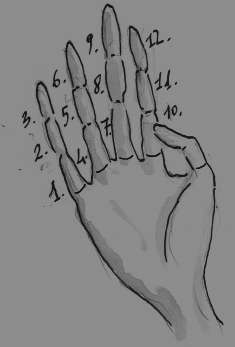
\includegraphics[width=0.3\textwidth]{figs/fingers.png}
\caption{“掐指一算”}
\end{figure}

在远古时代，用手指计数是再自然不过的选择——手指是人类最早的“随身计算器”。
它帮助人们轻松应对日常计数需求，如记录牲畜数量、物品交换量，推算季节与节气，安排农耕节日等活动。
由此，一个从身体到符号的过渡被打开：手指的结构成为进制与位权的直观原型。

手指的构造与多种进制系统有着天然的联系。稍加留意，我们就能找到十进制、二十进制、十二进制等计数法，都与人体的结构息息相关。

十进制(Decimal System)是最常见、最自然的计数方式，与双手十指一一对应。十进制系统在全球的广泛使用，源于人类天生拥有十根手指的解剖学特征。正如爱德华·卢卡斯所言，这是“自然界的一个偶然事件”​。

十二进制(Duodecimal System)则更为灵活。除大拇指外，四根手指各有三段指节。一只手的大拇指轮流指向这些指节，便可以计数1到12。这种方法在古代美索不达米亚和古埃及被广泛应用，至今仍深深植入与我们的时间和角度计数系统中，如12小时制和一年12个月。

六十进制(Sexagesimal System)则更加复杂，它结合双手来计数：一只手计12（与十二进制相同），另一只手则记录12的倍数，五轮12等于60。
这种方式最早诞生于古巴比伦，并延续至今，仍清晰地存在于我们熟悉的体系中：一小时60分钟，一分钟60秒，以及圆周360度的划分。

二十进制(Vigesimal System)进一步扩展了身体的范围：一些古代民族不仅用手指，还加上脚趾来计数。中美洲的玛雅和阿兹特克文明，以及西非和欧洲部分地区，都曾采用以20为基数的计数法，可谓“全身皆为算盘”。

二十进制的痕迹在许多语言中依然清晰可见。英语中的“score”（意为20）便是这一传统的遗存。
例如，莎士比亚在《圣经》英译本中使用“three score and ten”（20的3倍加10，表示70岁)来指代古稀之年；林肯在《葛底斯堡演讲》中使用“four score and seven years ago”(20的4倍加7，表示87年前的历史。一百年后，马丁·路德·金在其著名的演讲《I have a dream》中说“Five score years ago”​（20的5倍，即100年前）​。

英国也曾长期沿用\emph{12 与 20 进制结合}的货币系统：1英镑=20先令，1先令=12便士。1971年，英国才正式改为十进制货币系统：1英镑=100便士，先令在1990年后彻底退出流通。

在法语、丹麦语和巴斯克语中，同样能见二十进制的痕迹。法语数词从quatre-vingts(80)​到quatre-vingts-dix-neuf(99)，均以20为基数组合。同时，这些语言中还混杂了六十进制的痕迹，如数词soixante(60)到soixante-dix-neuf(79)。

手指不仅是身体的一部分，还是人类最早的天然计算工具。它帮助我们理解和组织世界，并为现代数学中的位值制和进制系统提供了最初的灵感。直到今天，人们在进行简单计算时仍会不自觉地“掐指一算”——那不仅是一种习惯，更是一段跨越千年的文明记忆。

\subsection{荒岛上的自然教育，人类数字文明的缩影}

设想一次航海探险中，你遭遇风暴，不幸漂流到一座无人岛。  
没有手表，没有手机，也没有任何现代工具。  
很快，一个原始而紧迫的问题摆在你面前——如何计算时间？如何记录每天收集的食物？  
在这样的环境里，你必须重新学习如何用最简单的方式去“数”、去“记”。  
而这段假想的经历，正是早期人类发明和发展数字的真实缩影。

\subsection*{手指计数：最简单的工具}
你的第一反应，或许就是用手指计数。  
十根手指是最天然、最便捷的“计算器”，可以帮助你记录每天捕到的鱼、采摘的果实数量。  
这种方法简单而直接，几乎不需思考。  
但很快你会发现它的局限——当数字变大，或需要记录更多的信息时，手指显然不够用。  
更重要的是，手指计数无法保存这些数据，一旦忘记，你的记录便随之消失。

\subsection*{刻痕计数：更长久的记录方式}

为了让记录更持久，你开始在岛上的树木或石头上刻下痕迹。  
每一道刻痕代表一天的过去，或一次捕猎、采摘的成果。  
随着时间推移，这些痕迹渐渐形成一个记录时间和活动的系统。  
刻痕计数虽然简单，却比手指更加持久、可靠，也能应对稍微复杂的需求，比如记录日期或特定的事件。  
然而，当刻痕越来越多，管理和读取它们变得越来越困难。  
于是，一个新问题出现了：有没有更便捷、更灵活的方式，能让信息被更好地保存与传递？  


\subsection*{结绳记数：更高级的记数法}
幸运的是，你在岛上找到了一根绳子，这给了你一个新的选择结绳记数法。  
你开始尝试在绳上打结，用结的形状、位置和数量来表示不同的信息：一天、一件事，或一批收获。  
与刻痕相比，结绳更加灵活、可携、可传递，也能更清晰地编码不同含义。  
这不仅是一种实用的工具，更是一种“符号化”的思维跃迁——数量开始脱离具体现象，成为可以被“编码”的信息。  


你在荒岛上的探索，正是人类数字文明进化的缩影。无论是刻痕还是结绳，这些方法都体现了人类从最初的物理标记到复杂符号系统的演化路径。通过这些最自然的“计数实验”，你逐步学会了如何记录、比较和计算。
这不仅是个人的“自然教育”，也是数字发明的最初动力让生活更加便捷和高效。


\section{数字的位值系统}

在人类早期文明中，手指计数、结绳与刻痕已被广泛用于记录数量。  
但随着社会复杂度提升，这些方法在面对大数或连续运算时，逐渐显得笨重而低效。  
于是，更加抽象的符号系统应运而生，催生出{\bf 位值制}——一种以“符号位置”表达“数值权重”的革命性思想，使复杂数量得以用有限符号清晰表示与计算。



举个直观的例子，可以用两串珠链来理解位值的含义。  
假设每串都有10颗珠子。  
若只是把两串珠子简单相加，最多只能数到20——这对应于“加法式记数”的思维。  
但若让一串代表“个位”，另一串代表“十位”，情况立刻不同：每动“十位”一粒，就相当于数量增加十倍。  
于是，两串珠链可以组合出$10\times10=100$种不同的状态。  
同样的珠子，通过“位置赋权”，计数范围便从“加到二十”跃升为“组合到一百”。这正是位值制的核心——位置决定权重。



早期的计数系统普遍采用{\bf 加法规则}。  
例如，在古巴比伦的泥板上，数字“1”用一个符号表示，“2”用两个相同符号，“3”则用三个相同符号——数值靠符号的重复来体现。

大多数古代文明在表示前三个数字时，都采取了同样的“重复记号”的计数方式。中文的“一、二、三”、钟表盘上的罗马数字“Ⅰ、Ⅱ、Ⅲ”、古印度与玛雅数字皆是如此。  
可是，从数字“4”开始，所有的文明就都放弃了这种重复。为什么呢？  

心理学研究发现，人类的数感对少于3的数字有天然的反应，几乎不需计算就能分辨1到3。  
但当数量超过这个范围时，就需要额外计算。  
想象一下，如果数字13要靠十三个“1”来写，光数清就要花好几秒。  
既低效又容易出错——根本无法一眼分辨是12、13还是14。

罗马数字对重复做了一些改进：V代表5，X代表10，L代表50，C代表100。  
小符号加在右边表示加法（VI=6，XI=11），放在左边则代表减法（IV=4，IX=9）。  
这种方法直观，但规则较多，记忆和书写都不轻松。

早期加法型记数虽然直观，但在表示大数时效率极低。  
例如，1888要写成MDCCCLXXXVIII， 若要表示一百万，就得写出上千个M。这类体系在规模扩大后难以使用。

随着文明的发展，人们陆续发明了更高效的计数方法，其中最具革命性的便是{\bf 位值制}。  
古巴比伦的六十进制、中国的筹算以及印度—阿拉伯体数字系，都在不同路径上孕育出这种思想，并最终汇聚为现代十进制体系。

位值制的核心在于——符号的位置决定了其“权重”。  
同样的数字“1”和“2”，写作“12”与“21”时意义却完全不同。  
从数学上说，十位权重是$10^1$，个位权重是$10^0$。



位值计数法最大的优点是简洁。 
只用0到9十个符号，就能表达任意大的数。  
比如$10^{100}$这个天文数字，只需“1”后跟100个“0”——规模呈指数增长，而长度只线性增加。

位值制不仅提高了数字的表示效率，还体现了数字的{\bf 对数增长}特性，即随着数值的增大，表示所需的符号长度不是线性增加，而是呈对数增长。例如，表达$10^{100}$所需的符号长度约为$\log_{10}(10^{100})=100$——长度的增加远小于数量规模的增长。
一般地，表达任意整数 $x$所需的符号个数约为 $\lfloor \log_{10} x \rfloor + 1$。 



从信息论的角度来看，位值系统是最简洁、甚至接近最优的表示方式。  
{（信息论视角：最短码长度$\approx -\log p$。）}\emph{它也成为现代信息处理与计算架构的基础。}  



位值制的出现，标志着人类计数方式的重大转变。  
它将“重复符号”的直觉提升为“位置赋权”的概念，使得让表达与计算都获得了指数级的效率提升。  
这一思想也深刻影响了现代计算的底层逻辑。  


\subsection{位值制与对数增长在现代计算机中的应用}
  




在计算机科学中，二分查找是一种常见而高效的方法。  
当我们在一个排好序的数组中寻找目标元素时，所需的步骤并不随数组长度线性增加，而是与它的对数成正比。  
换句话说，即使数据量大到天文级，经过几百次比较，也足以定位到目标。  





我们每天使用的互联网链接，其实就是位值制思想的现代延伸。  
一个短短的URL，就能在海量的信息世界中精准指向某个资源。  
几行字符之所以能对应整个网络空间，正是“位置与权重”的逻辑在发挥作用。
  

想象一下，当我们在网络上搜索一条信息时，面对的数据量可能高达EB甚至ZB级。  
但只要拥有那串对应的URL，就能几乎瞬间到达目标页面。  
这正体现了“对数式增长”的特征：即使信息空间成倍扩张，定位时间几乎不变。






从工程角度看，URL 的长度与整个网络的规模大致呈对数关系。  
也就是说，用较短的字符串，就能索引到巨大的信息空间。  
这种“以小驭大”的结构，正体现了对数思维在信息系统中的力量。



IPv4和IPv6的设计，是“对数式扩展”的另一生动实例。  
{\bf IPv4} 使用32位二进制表示，通常写成四段十进制形式（如192.168.1.1），每段对应8位。  这样一串数字，实际上就是全球网络中唯一的地址标识。

32位二进制可生成约$2^{32}$，也就是{\bf 43亿}个地址。  
在互联网早期，这个数字似乎已经“多得用不完”。  
然而，随着互联网的迅速扩展，特别是物联网（IoT）设备和移动设备的广泛普及后，IPv4的43亿个地址空间将很快耗尽。  


于是，{\bf IPv6} 应运而生。  
它使用{\bf 128位}二进制数，由八组16进制数构成(如 2001:0db8:85a3:0000:0000:8a2e:0370:7334)。
这种表示能生成$2^{128}$，约{\bf $3.4 \times 10^{38} $} 个唯一IP地址。  
这意味着，即使为地球上每一粒沙子编号，也仍然绰绰有余。  
这样的容量，足以支撑未来数十年甚至更长时间的联网设备的需求。 








从IPv4到IPv6，只是位数从32扩展到128，  
但可用地址数量却从43亿跃升到$10^{38}$量级。  
位数的提升带来了指数级的扩展，同时保持了表示形式的简洁。  
这就是对数增长的魅力所在——少量的扩展，换来巨大的可能。  




\subsection{数字：从具象到抽象}

几千年来，人类一直在探索如何建立数与物的对应关系。现代数字系统的形成，正是这种探索的延续。
当人类掌握了计数，数字的使用似乎变得顺理成章——这或许就是“自然数”名称的由来。  
不过，如果仔细思考就会发现，数字并非天然存在，  
而是人类通过经验与思考“发明”出来的一种抽象语言。

无论是人类早期在骨头及木棍上有序地刻下划痕，还是通过结绳、在容器中放置物品来纪录数量，这些方法都体现了最初的“符号化”意识。 
随着时间的推移，抽象的数字逐渐与自然中的具体物体分离。同一个“3”，既可以表示三只羊，也可以代表三天或三笔账。从此，数字不再依附于物，而成为可独立思考的抽象概念。




从那时起，数学研究的对象不再局限于与具体事物相关的几何图形和数量。 
数字与形状开始被独立地思考，它们之间的关系也可以被重新定义。  
这种研究对象的转变，最终带来了方法论上的一次{\bf 革命}。



抽象有助于让知识得以迁移与延展，，也让我们在理解上获得新的视角。  

\section{初等数学时期：从计算到推理}
公元前5世纪开始，数学进入了“初等数学时期”。  
这一阶段的探索更系统、更深入。
欧几里得几何与代数方程的研究使得“数—形”关系走向严谨，  
算术、几何、代数与三角等分支逐步成形，标志着早期数学结构的建立。这一时期的核心转变在于：从求值走向论证，从技巧走向体系。

数学作为学科经历了漫长的演化。  
起初，数学的诞生是为了解决生活中的实际问题——计数、测量、交易、管理时间等。  
公元前5世纪之前，埃及与美索不达米亚的数学更多依赖于经验与操作，  
主要服务于土地测量、建筑工程、会计管理与天文学等计算需求。


这种以算术与几何为主的“实用性数学”常被称为“史前数学”。  
它围绕日常需求展开而较少抽象推理，  
也正因如此，才凸显出随后“转向证明”的意义。


古代数学多服务于实践，而希腊学者把关注点转向命题的\emph{可证性}。  
等腰直角三角形三边皆为整数的设想，化为方程 $2x^2=y^2$。  
他们尝试穷举未果，转而假设互素并通过分类奇偶导出矛盾，结论是无解。  
\emph{由此，数学的目标从“得到一个数”转向“给出必然理由”，由“如何计算”迈向“为什么如此”。}  
这一转折打开了更广阔的对象与方法空间。
正因如此，教科书常从公元前5世纪的希腊讲起，  

原文：
在公元前5世纪的希腊，毕达哥拉斯学派提出了这样一个问题：找出一个等腰直角三角形，使其三边的长度都是自然数。


语气更课堂化，保留提问式导入。


在此背景下，毕达哥拉斯学派提出了这样一个问题：  
能否找到一个等腰直角三角形，使三边长度都是自然数？





设等腰直角三角形的直角边长度为 $x$、斜边长度为 $y$。由毕达哥拉斯（勾股）定理，~$y^2=x^2+x^2$。  
于是问题归结为：找出自然数 $x,y$ 使
\begin{equation}\label{eqn}
2x^2=y^2.
\end{equation}


\begin{table}[htbp]
\centering
\caption{4以内$x$与$y$的所有可能性}
\begin{tabular}{|c|c|c|c|}
\hline
$x$ & $y$ & $2x^2$ & $y^2$ \\
\hline
1 & 1 & 2 & 1 \\
\hline
1 & 2 & 2 & 4 \\
\hline
1 & 3 & 2 & 9 \\
\hline
1 & 4 & 2 & 16 \\
\hline
2 & 1 & 8 & 1 \\
\hline
2 & 2 & 8 & 4 \\
\hline
2 & 3 & 8 & 9 \\
\hline
2 & 4 & 8 & 16 \\
\hline
3 & 1 & 18 & 1 \\
\hline
3 & 2 & 18 & 4 \\
\hline
3 & 3 & 18 & 9 \\
\hline
3 & 4 & 18 & 16 \\
\hline
4 & 1 & 32 & 1 \\
\hline
4 & 2 & 32 & 4 \\
\hline
4 & 3 & 32 & 9 \\
\hline
4 & 4 & 32 & 16 \\
\hline
\end{tabular}
\label{tab:example}
\end{table}


让我们先在 $x,y\le 4$ 的范围内试探所有可能（见表~\ref{tab:example}）。


在上述所有情况下，$2x^2$ 都不等于 $y^2$。  
我们当然还可以在更大的数字范围内继续寻找，事实上，毕达哥拉斯学派很可能寻找了很久，却没能找到解。
于是，一个判断出现了：解可能不存在。  
如何说服自己？穷举不可行，因为这样的数对有无穷多个。  
即便检验到 $10^3$ 或 $10^6$，也无法保证更大范围没有解。

据此，我们把数对$x,y$分成以下3种情况:
\begin{enumerate}
\item $x,y$都是奇数;
\item $x$是偶数，$y$是奇数;
\item $x$是奇数，$y$是偶数;

\end{enumerate}


先看第一种情况：$x,y$ 都为奇数。则 $y^2$ 为奇数，不可能等于必为偶数的 $2x^2$。  
同理，第二种情况：$x$ 为偶数、$y$为奇数，也不成立。  
第三种情况：$x$为奇数、$y$为偶数。若 $2x^2=y^2$，则 $x^2$ 为奇，而 $y^2/2$ 为偶，二者不可能相等。


因此，不存在自然数 $x,y$ 使得~\eqref{eqn} 成立。


这里，毕达哥拉斯学派选择了逻辑而非穷举。  
他们通过分类讨论与推理，证明了无论 $x$ 和 $y$ 的奇偶性如何，$2x^2=y^2$ 都不可能有整数解。

原文：
这一问题的解决在数学史的发展上具有划时代的意义。它的革命性不仅在于其对未来数学的巨大影响，还在于其抽象性及解决的方法。相比于美索不达米亚泥板上铭刻的诸如“将1152000份粮食除以7份”的具体问题，毕达哥拉斯学派的问题更为抽象：美索不达米亚的会计师关注粮食的数量，而毕达哥拉斯学派的问题仅涉及数字本身。同样，他们处理的是抽象的几何形式，而非具体的三角形田地。从从粮食的份数到数字，从实际的土地测量转向几何学的抽象思考，迈向抽象这一步的意义不可小觑。田地的面积无非几平方千米，而抽象的几何对象则可以轻松超越这一尺度，进入无限的范围。



这一问题的解决在数学史上具有划时代意义。  
它的{\bf 革命性}不仅在于影响广泛，也在于其抽象性与解决方法。  
相比于美索不达米亚泥板上铭刻的诸如“把~$1152000$份粮食除以7”的具体问题，  
毕达哥拉斯学派的问题面向抽象数字本身。  
同样，他们处理的是抽象的几何形式，而非具体的三角形田地。
由“粮食份数”到“纯数字”，由实际的“土地测量”到“几何抽象”思考，  
这一步迈向抽象的意义不可小觑，它让研究对象超越尺度，指向无限。


古希腊数学家不再满足于计算结果，而是重视推导过程。  
通过严谨的逻辑推理，他们逐步建立了数学证明方法与公理体系。


这一从“计算”到“推理”的转变，常被视为数学的真正诞生。  
由此，数学从日常的计算工具走向以推理与抽象为核心、具有高度抽象和严谨逻辑的独立学科。

一个平方数不可能是另外一个平方数的两倍——这个由毕达哥拉斯学派在 2500 年前得到的结论，至今在数学上仍占有重要地位。它证明了，一个直角边为 1 米的等腰直角三角形，斜边的长度为$\sqrt{2}\approx1.414$，但这个数不能通过两个自然数 $y$ 和 $x$ 的比值得到。这揭示了，某些几何关系不能仅依靠自然数的四则运算(加、减、乘、除)获得到，并暗示了更广泛的数系——实数的存在。这一发现让数学进入了一个全新的领域——从实际问题中抽象出纯粹数学对象，并通过推理得出结论。

虽然这一发现具有革命性，但毕达哥拉斯学派并没有进一步发展出实数的概念。
对他们而言，这一结论动摇了他们对"万物皆自然数"的信仰，甚至引发了哲学上的困惑与争议。然而，几百年后，这一发现启发了数学家们发展出实数理论，为数论和分析学的诞生奠定了基础。


古希腊数学家的贡献不止于发现了一些几何定理和代数法则。  
更重要的是，他们发展了数学思维的方式：演绎、证明与公理化。  
由此，数学从经验性工具转为一门严谨的科学。  
这一传统不仅奠定了现代数学的基础，还持续推动了后世的科学进步。


希腊数学的影响并未止步于欧洲。  
中世纪的阿拉伯数学家翻译了希腊经典，并引入了印度的十进制与“零”的概念。  
阿尔·花剌子密（al-Khwarizmi）等数学家对代数学的发展做出了巨大贡献，他的著作奠定了代数理论的坚实基础。（"algorithm"一词即源于其姓名的拉丁化形式。）


中国的《九章算术》与印度的早期代数成就，也为初等数学的发展增添了重要内容。  
中国古代数学强调实用性，广泛服务于农业、建筑与税务管理；而 印度数学则对数论和代数的早期发展做出了杰出贡献。  
不同文化的数学成果，共同塑造了初等数学的基础版图。


这一时期大致涵盖公元前5世纪至17世纪前的数学发展。 数学由应用走向抽象，古希腊在几何与数论中搭建起推理与证明的体系。  
这一阶段的数学成就不仅构成了今天中学数学的主要内容，还对现代数学的基本理论结构产生了深远的影响。

\section{近代数学时期：变量、函数与微积分}
原文：
初等数学时期确立了严谨推理的传统，而从17世纪开始，数学面临着新的挑战和机遇。随着资本主义的崛起和工业革命的推动，数学进入了一个全新的阶段变量数学时期。




初等数学时期确立了严谨推理的传统。  
而从17世纪开始，新的挑战与机遇接踵而至：资本主义兴起，工业革命推动需求增长。  
在这样的背景下，数学进入了一个新的阶段——以变量为核心的时期。







这一时期的数学研究，从静态图形与数量逐步转向对变化与运动的刻画。  
为此，引入变量与函数，成为描述与分析变化的关键工具。  
换句话说，我们开始用“量随量而变”的视角看问题。




牛顿与莱布尼茨分别独立创立了微积分，标志着数学史上的重要转折点。  
微积分建立了一套精确刻画连续变化与瞬时变化的数学框架，使“变化”这一概念首次能够被计算和推理。  
它能有效处理速度、加速度、曲线下面积等问题，成为研究运动与变化的核心方法。  
牛顿借此为万有引力定律提供了坚实的理论基础，莱布尼茨则将微积分符号化并推广至欧洲，使其成为普遍的科学语言。   
自此，数学不再局限于静态图形的描述，而是迈向对连续变化的系统分析，开启了数学分析的新篇章。




解析几何的诞生是这一时期的另一个重大突破。  
笛卡尔引入坐标系，把几何与代数结合，使复杂图形、运动及空间关系可用代数方程精确刻画。  
借助笛卡尔坐标系，曲线与直线的关系能够用代数表达，许多问题因而被显著简化。  
因此，解析几何既为物理学中的动力学提供有力工具，也为现代数学的发展铺平了道路。


近代数学时期的另一个重要分支是概率论。  
它最初由费马和帕斯卡为研究赌博中的随机事件而建立，但很快超越了这一背景，成为刻画不确定性与随机规律的重要工具。  
与此同时，费马还在数论领域提出了许多关于素数与整数关系的深刻问题，激发了后世数学家的广泛研究。  
欧拉、拉格朗日等人进一步推动数论的发展，深入探讨了代数结构与数的基本性质。









与此同时，分析学在微积分基础上发展为这一时期的核心数学分支。  
通过函数与极限概念的引入，数学家能够严格处理无穷小与变化中的量，分析学由此成型。  
数学分析不仅解决了古希腊时期悬而未决的部分几何难题，还广泛渗透进物理学、天文学与工程学，极大地推动了科学的进步。


原文：
总的来说，近代数学时期不仅为数学的进一步抽象化奠定了基础，还通过微积分、解析几何和概率论的兴起，彻底改变了人类对世界的理解方式。
数学在这一时期的变革性进展，成为了现代数学发展的根基，也为科学技术的进一步进步提供了强有力的工具。


\section{现代数学时期：抽象、结构与计算}


近代数学已经建立了处理变化与连续性的工具。  
进入19世纪中叶，数学迎来了又一次深刻的变革——从经验方法走向高度抽象与系统化。  
这一时期被称为现代数学时期，它标志着数学开始重新思考自身的基础与结构。




这一时期的数学不仅延续了分析学的发展，还引入了全新的几何与代数思想。  
代数、几何和分析等传统学科都发生了质的飞跃，研究对象与方法逐步走向更高层次的抽象。  
这种趋势让数学从分散的知识体系，演化为一门更系统、更具普适性的科学。


现代数学的一个显著特征，是对基础的重新审视与抽象概念的不断扩展。  
罗巴切夫斯基和黎曼创立的非欧几何，彻底改变了传统欧几里得几何的空间观念，提出了球面、鞍面等新的几何结构。  
它们揭示了更为广阔的空间与结构关系，也为现代物理提供了数学语言。  
与此同时，拓扑学在19世纪兴起，突破了传统几何的限制，成为研究连续性、边界与形态的重要工具。




现代数学的发展，也离不开对“无穷”与基础问题的深入研究。  
康托尔创立集合论，为研究无穷大小提供了严格的工具，使无穷大与无穷小的概念得以精确化，成为现代数学与数理逻辑的重要基础。  
这一理论不仅在抽象层面统一了数学，还引发了对数学自身根基的反思。  
希尔伯特、哥德尔等数学家的工作，使公理化体系进一步完善，也揭示了形式体系的可能与局限。




进入20世纪，统计学、拓扑学与泛函分析等新分支相继形成，使数学的结构更加多元，也更具应用性。  
它的影响力从理论研究扩展到物理、工程、经济等广泛领域，成为众多学科的共同语言。  


原文：
现代数学时期的另一个重要推动力是计算机的发明和信息技术的迅猛发展。20世纪中期，图灵、冯·诺依曼等科学家为计算机科学奠定了理论基础，计算理论逐渐成为数学的重要分支。计算机的强大计算能力使得复杂的数学问题得以快速求解，同时也极大地推动了数理逻辑和算法理论的发展，数学的潜能和边界更进一步发掘。{（一句话抽象：可计算/复杂度的边界塑造了"可做之事"。）}




现代数学的另一股强大动力，来自计算机与信息技术的兴起。  
20世纪中期，图灵与冯·诺依曼为计算机科学奠定了理论根基，使计算理论成为数学的新分支。  
计算机的的强大计算能力使得复杂的数学问题得以快速求解，同时也极大推动了数理逻辑与算法理论的发展，数学的可能边界进一步拓展。  





随着数学的抽象化与理论化趋势不断加深，它不仅深入自然科学的核心，也广泛渗透至信息、工程、经济与社会科学等多个领域。  
数学逐渐成为理解自然世界、构建模型与推动创新的核心力量，为现代社会的发展提供了持续动力。

原文：
总之，现代数学时期是数学高度抽象化、系统化的阶段。数学基础理论的发展、新分支的创立以及计算机技术的推动，使得数学成为现代科学技术发展的重要支撑。这一时期的数学不仅在理论上达到了前所未有的高度，还在实际应用中展现了巨大的潜力，为人工智能等新兴领域的发展奠定了坚实的数学基础。{（一句话抽象：变化、空间与不确定性三件套；AI 去向：优化、几何表示、概率图模型。）}




总的来说，现代数学时期是一个高度抽象化与系统化的阶段。  
基础理论的深化、新分支的涌现，以及计算机技术的推动，使数学成为现代科学与技术的重要支撑。  
这一时期的数学不仅在理论上达到了前所未有的高度，还在实际应用中展现了巨大的潜力，为人工智能等新兴领域的诞生与发展奠定了坚实的数学基础。


\section{三次数学危机}


在漫长的数学发展史中，曾出现过三次意义深远的危机。  
这些危机不仅揭示了当时理论体系的局限，更在反思与重建中推动了数学的革新。  
可以说，每一次危机的爆发与解决，都是数学向更高层次走去的契机，使它在逻辑与结构上变得更加严谨、更加成熟。

在漫长的数学发展历程中，曾出现过三次意义深远的危机，深刻地改变了数学的方向。这些危机不仅揭示了当时理论体系的局限，同时也成为推动数学革新的契机。每一次危机过后，数学都变得更加严谨、更加完善。



\subsection{第一次数学危机：无理数的发现}


第一次数学危机发生在公元前5世纪的古希腊，起因是毕达哥拉斯学派发现了无理数的存在。

毕达哥拉斯学派坚信“万物皆（有理）数”，认为一切量都可表示为两个整数的比值，即有理数。然而，当他们研究直角边长为1的等腰直角三角形时，意外地发现了一个矛盾：斜边的长度$\sqrt{2}$，无法写成任何两个整数的比。  


这一发现彻底动摇了毕达哥拉斯学派的数学哲学根基。  
无理数的发现说明，数的世界比他们想象得更复杂——  
并非所有量都能以整数比来表达。

这场危机的化解经历了漫长的探索。  
为避免直接面对这一困难，古希腊数学家转而以几何方式处理无理量。因此，在此后的很长一段时间里，几何在古希腊数学中被视为更高层次的研究形式，地位远高于代数。
直到十九世纪，戴德金和康托尔才为无理数建立严格定义，完善了实数理论。
这场危机让数学家首次意识到：数的概念需要被扩展。它促成了实数理论的诞生，也为后来的数学分析奠定了基础。

\subsection{第二次数学危机：微积分基础的争议}

第二次数学危机发生在17至18世纪，焦点在于微积分的基础问题。
牛顿和莱布尼茨各自独立地成功发明了微积分，虽然在实践上取得了巨大成功，但他们对“无穷小量”的本质缺乏严格的定义。

当时的数学家在使用微积分时，经常涉及“无穷小量”的概念。这些量被认为既不是零，又比任何正数都小，这在逻辑上难以自洽。贝克莱主教因此尖锐批评道：无穷小量不过是“已逝量的幽灵”。 

换句话说，微积分在应用中十分有效，但理论基础却不够坚实。数学家们意识到，要让这一工具真正站得住脚，必须为它建立更坚实的理论基础。




这一危机最终由19世纪数学家通过极限概念的严格化得以解决。

柯西、魏尔斯特拉斯等数学家建立了严格的极限理论，用$\varepsilon-\delta$语言重新定义了连续性、导数与积分等概念，彻底消除了无穷小量的逻辑困境，使微积分脱离了“模糊直觉”，  转而立足于严谨的逻辑框架之上。



自此，微积分终于拥有了坚实的理论基础，  
并催生出更广阔的分析学体系。  
数学也由此进入了以极限与连续性为核心的新时代。  


第二次数学危机的解决不仅使微积分获得了严格的理论基础，还推动了数学分析的发展，建立了现代分析学的基础。

\subsection{第三次数学危机：集合论与逻辑悖论}

第三次危机出现在19世纪末至20世纪初。  
这一次的问题不在计算方法，而在数学的根基——  
集合论在试图统一数学语言的过程中，却意外暴露出深层的逻辑悖论。






康托尔的集合论最初为数学提供了统一的语言与框架。  
然而不久之后，人们发现其中隐藏着令人不安的矛盾。  
最著名的例子是“罗素悖论”：  
设~$R$为“所有不包含自身的集合所组成的集合”，  
那么~$R$是否包含自身？  
若包含，则违背定义；若不包含，又应被自身包含。这形成了一个自我循环的逻辑困境，  
也让人们第一次意识到，问题已触及数学的根本。






这场危机的严重性前所未有。  
因为一旦集合论本身存在逻辑漏洞，那么建立在其上的整个数学体系都将岌岌可危。  
这不仅是一个学科的危机，更是关于“数学是否能够自洽”的根本挑战。






为应对危机，数学家们开始从根本上重建集合论。  
他们提出了多种公理化体系，其中最具代表性的是ZFC系统（策梅洛–弗兰克尔公理加选择公理）。  
这些公理通过严格限制集合的构造方式，成功避免了已知的悖论，让集合论重新获得了可以立足的逻辑基础。






与此同时，这场危机也催生了数理逻辑的兴起。  
希尔伯特提出“形式主义纲领”，试图以符号与公理体系为数学建立绝对可靠的逻辑基础。  
然而，哥德尔的不完全性定理揭示：任何足够复杂的体系，都无法在自身内部证明自己的完备性。    
尽管如此，这一系列研究极大地拓展了数学思想的边界，  
并催生了现代逻辑与计算理论的诞生。






第三次危机的解决虽然仍留有未解之处，  
却极大地拓展了数学基础理论的版图。  
它为现代逻辑学、集合论和计算理论奠定了根基，  
并揭示了形式系统的边界与复杂性的极限。  







纵观这三次数学危机，我们看到一个清晰的规律：  
每一次危机既暴露了旧体系的不足，却也带来了新的突破。  
数学正是在一次次的质疑、反思与重建中变得更加严谨与深刻。  
可以说，危机即机遇——正是在矛盾与困惑中，迫使我们重塑概念与方法，使数学不断获得新的生机。由此可见，数学乃至整个科学的进步从不是直线，而是一种在困惑中求解、在矛盾中前行的过程。
正如三次数学危机所揭示的那样——危机即机遇，  
每一次反思与重构，都是通向更深理解的新起点。


\section{小结}

回顾数学的发展历程，我们可以清晰地看到：  
这是一条由具体走向抽象、由经验走向理论、由分散走向统一的演进之路。  
这不仅是知识的积累，更是人类思维方式的演化。

从最初的计数需求到现代数学的高度抽象，  
数学经历了四个主要阶段：  
萌芽时期奠定了数字表示的基础；  
初等数学时期确立了严谨推理的传统；  
近代数学时期发展了刻画变化与连续性的工具；  
现代数学时期则实现了抽象化与系统化的飞跃。

三次数学危机虽然为数学的发展带来了严峻挑战，  
但正如历史所示——危机往往孕育机遇。  
无理数的发现扩展了“数”的边界；  
微积分基础的严格化奠定了现代分析学的框架；  
集合论悖论的研究则推动了数理逻辑的兴起。  
数学正是在一次次危机中实现了自我成长与超越。

更重要的是，这一历程也为现代人工智能的发展提供了深刻启示。  
从位值制的编码思想到几何的空间表示，  
从概率论中的不确定性处理到逻辑的形式化推理，  
数学的每一个核心概念都在人工智能中找到了新的生命与实现方式。  
换句话说，AI的发展，是数学思维的一次技术化延伸。

数学不仅是一门抽象的学科，更是人类理解与改造世界的核心工具。  
如果我们回望历史，从古代的天文观测到现代的计算机科学，  
从艺术创作到科学发现，  
数学的影响始终深藏于人类文明的每一次跃迁之中。






在漫长的文明史中，数学贯穿了人类创造力的每一次跃迁。  
达·芬奇以数学比例构筑艺术的平衡；  
哥白尼以计算颠覆宇宙观；  
牛顿用微积分统一天地运动；  
巴赫以十二平均律谱写音乐秩序；  
孟德尔用统计揭示遗传规律；  
爱因斯坦以方程重新定义时空；  
图灵和冯·诺依曼则将数学思想转化为计算机与人工智能的核心。  
无论是艺术的和谐还是科学的突破，数学都在背后默默支撑着人类的理解与创新。






这些例子表明，数学不仅是科技发展的基石，  
更是人类文明进步的重要推动力。  
进入人工智能时代，这一点尤为突出——  
从机器学习的统计基础到深度学习的优化算法，  
从逻辑结构到计算复杂度，数学为AI提供了不可或缺的支撑与方向。





理解数学的发展史，有助于我们更好地把握人工智能发展的脉络和方向。  
正如数学不断突破自身的边界、走向更高层次的抽象，  
人工智能也在不断突破技术的极限，迈向更深层的智能。  
数学发展史告诉我们：每一次重大的突破，都源于对基础概念的深入思考与对现有理论的勇敢质疑。  
这种精神对于人工智能的发展同样具有重要的指导意义。




在学习与研究人工智能的过程中，我们既要扎实掌握数学的基础，  
也要具备历史的眼光与哲学的思维。  
唯有如此，我们才能在人工智能的发展道路上走得更远，
创造出更加智能、更加有益于人类的技术成果，让科技真正服务于人类智慧的拓展与福祉。





数学的发展史展现了人类智慧的演进，也为我们理解和发展人工智能提供了宝贵的经验和启示。  
从"现象—抽象—启发—取舍—去向"的学习闭环中，我们不仅能够掌握数学知识，更能够培养科学思维，为未来的创新和发展奠定了坚实的基础。



